\section{Discussion}

%interpretations!!\\

%Compare with data/theories from other people, theory and other literature. references!!\\
%re-plot some of the data in another fashion to illustrate the main points.\\
%Plot data from other students' report.\\
%References!!\\

\subsection{Evolution in growing sea ice}
Temperature data recorded at the weather stations placed on the ice, proves that the cold air temperatures measured by the harp shown in Figure \autoref{temperatureharp2} is also quite accurate measurements of the air temperature \textcite{Weather}. Its important to mark that the harps sensor is on a different height, and is more a measurement of the surface temperature, than air temperature per say, which would explain the measurement differences. In general it can be said that for the cold temperatures measured they match quite good. For the very warm temperatures measured, the deviation is something else. The highest temperature that the harp recorded of \SI{3}{\celsius} cannot be found in the weather station temperature measurements at all. An explanation for this would lie in that the sensors on the weather station is shielded against radiation from the sun, while the sensors on the harp isn't. Therefore the recorded high temperature is due to sun rays heating up the sensor. Another proof of this is the sudden drop in the measured temperature at around 13:00. Manual observations from \textcite{Weather} shows that there was an increased cloud coverage at that time. The cloud coverage would block the direct sunlight from reaching the temperature sensor, and that is why the data "suddenly" looks more reasonable. Other than that, the temperature evolution shown in Figure \autoref{temperatureharp2} shows that we have cold enough ocean water for sea ice formation to occur, and when compared with the temperature measurements from Table \autoref{Ice_core} they are the same. \\
\\
Figure \autoref{liquidfractionharp2} shows a clear evolution of how the liquid mass fraction is decreasing in the beginning at the surface, implying that here is sea ice forming. From the same figure it is possible to observe that the quickest sea ice growth at the very start, and at around 01:00 on the 19. of April. It is also possible to observe that we have very little increase in the sea ice thickness after the first night. A possible explanation for this is that the air temperatures that were recorded by the weather stations show that the temperatures increased over the following days \textcite{Weather}, and thus the temperature gradient is smaller between the underlying ocean and the atmosphere above. Based on that we can assume that there is a strong correlation between the heat flux through the ice and vertical ice growth. This was also proven by the harp experiments done in the 2016 AGF-211 cruise \textcite{2016icegrowth}.\\
\\
After the snow experiment was started one can from Figure \autoref{liquidfractionharp2} clearly see the increase of the liquid fraction at the top of the harp due to the flooding that happened after loading the ice with the snow. Furthermore, the same figure shows that, as time passes the whole upper column freezes up. Looking at the bottom left image in Figure \autoref{experiment_evolution} one can also see that this refreezing has taken place, as the ice now has the same colour as the ice around it. Also when looking at the end of Figure \autoref{liquidfractionharp2}, it shows that the refreezing occur both from above, and from below. When comparing this with the temperature Figure \autoref{temperatureharp2}, it shows that the entire column gets the same temperature as the water below when the flooding occurs. The whole column does have any notable changes in temperature after this. This is expected, as the temperature difference between the air from the weather stations \textcite{Weather}, and ice is not large at all.\\
\\
The salinity evolution in Figure \autoref{salinityharp2} clearly shows when viewed in comparison with the sea ice forming in Figure \autoref{liquidfractionharp2} that the most brine release is when we have the most sea ice forming. As there is less sea ice forming later on, there is also less brine release into the ocean underneath. In other words it is a beautiful correlation between two evolutions. We can also see the salinity increase at the top due to the flooding event, and the following salinity decrease over time. What I cannot explain is where this salinity disappears to, as it does not propagate downwards due to for example gravity dragging the it down (gravity drainage). There was a substantial snowfall during the last part of the experiment, and the impact of that can be seen in the bottom right image in Figure \autoref{experiment_evolution}. A possible explanation is that the new fresh snow which has salinity of 0 causes the salinity to be dispersed in the new snow, instead of draining down.\\
\\
During the experiment there was an unexpected visit by a curious seal, and its impact can be visually seen as from the first image in Figure \autoref{experiment_evolution}. In the liquid mass fraction evolution, Figure \autoref{liquidfractionharp2}, the impact of this incident can be seen at just before 12:00 on the 19. of April UTC on the surface wire. It takes some time until we can see a salinity increase at around the same time stamp at the same place in the salinity evolution Figure \autoref{salinityharp2}, as seal only created a small flooding.\\
\\ 
As there was no sea ice below the second sensor, all of the values below this must be taken with a huge grain of salt. The equations used for calculating the salinities, and liquid mass fractions is based around a value ($Z_0$) which as stated earlier represents the point where ice starts to form. As there was no sea ice forming on the bottom four harps, all of these values that the figures for salinity and liquid mass fraction present for the depth below \SI{10}{cm} are most likely wrong. To eliminate these errors from the plot would require a lot more fine tuning of the codes used for interpreting and plotting the data, and is something that can greatly be improved. 
%There is a nice gradient at towards the end, where it is possible to see how the ocean heat flux propagates through the ice. The two previous AGF-211 Cruises has also proven that snow has an isolating effect.



\subsection{Salinity evolution in snow on ice}

From figure \autoref{liquidfractionsnow} it is easy to see that the rise of brine happens in two different speeds, one is through flooding the other is through capillary rise. The flooding happens fast and the capillary rise takes time. It is however evident that both of these have a somewhat linear shape. Taking this into account and the fact that the flooding can be calculated using Archimedes principle, along with Darcy's law and the Young-Laplace equation, it should be possible to make an analytical model of the process.\\
\vspace{0.4cm} 

To find the pore size, I need some simplifications of the snow. Assuming that the snow is made up of spheres, I can study this from a mathematical view. Close packing is used to describe the most dense setup of spheres in a cube.\\
\\
From this I can find the smallest pore size that can exist in this setting. Since there is two whole circles in this, and four halves of an open space, it is easy to find the area of this open space:
\\
\begin{figure}[ht]
	\begin{minipage}{.4\textwidth}
     \centering
        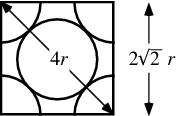
\includegraphics[scale=0.7]{ClosePackingFace}\\
     Sketch from \textcite{ClosePacking}
  \end{minipage}\quad
  \begin{minipage}[scale=0.8]{.4\textwidth}
    \begin{align}
        \text{A}_{\text{square}} &= (2\sqrt{2}r)^2 = 8r^2\\
        \text{A}_{\text{circles}} &= 2\pi r^2\\
        \text{A}_{\text{empty}} &= r^2(8-2\pi)\\
        \text{A}_{\text{opening}} &= \frac{r^2(8-2\pi)}{2}
    \end{align}
  \end{minipage}
\end{figure}

Assuming for simplicity that the pores are circular we can find the radius by:
\begin{equation}
    \text{R}_{\text{c,min}} = \sqrt{r_{\text{grain}}^2\left(\frac{4}{\pi}-1\right)}
\end{equation}
Finding the biggest possible pore is a bit more cumbersome as we have to take into account that we are working with snow, which has a tendency to stick together and not fall down in the tightest spot possible as a friction-less sphere would do. However, I am still assuming that the biggest likely opening would occur in what they in crystallography call a point defect, this is where one whole sphere is missing from the close pack. Since the snow is often moved around by snow, it is not so drastic to assume that any bigger hole would eventually be filled by a grain of snow. Using the same logic as before we find:
\begin{equation}
    \text{R}_{\text{c,max}} = \sqrt{r_{\text{grain}}^2\left(\frac{16}{\pi}-4\right) + r^2}
\end{equation}
\\
The values for the viscosity of saline water at $0^{\circ}C$ is around $2 \text{Kg}/m/s$ \textcite{Viscosity_1}, \textcite{Viscosity_2}. The surface tension for saline water at $0^{\circ}C$ is around $77 N/m$ \textcite{SurfaceTension_1}, \textcite{SurfaceTension_2}. We are working in subzero temperatures, however as the model still needs to be tuned to the permeability of snow, this should not be to much of a problem.\\
\\
Now we have everything needed for using Darcy's law (equation 1.1) and the Young-Laplace equation (equation 1.3), except permeability.\\
\\
Using the average between $R_{c,min}$ and $R_{c, max}$ a model running 4 days was tuned to matched the time where we assumed capillary pressure was the driving force. (08.00 - 20.00 at 19.04). This gave a permeability value of: $0.5^{17}/3.4$. Afterwards the model was run with a random set of 1000 pore radii with a normal distribution, with a mean on the average, and a standard deviation with half the distance from the mean to $R_{c,max}$. The values are forced to not go lower than $R_{c,min}$, but are allowed to go bigger than $R_{c,max}$. To make it more stable the results where averaged over 10 runs. \\
this gives us a plot like this:

\begin{figure}[h!]
\centering
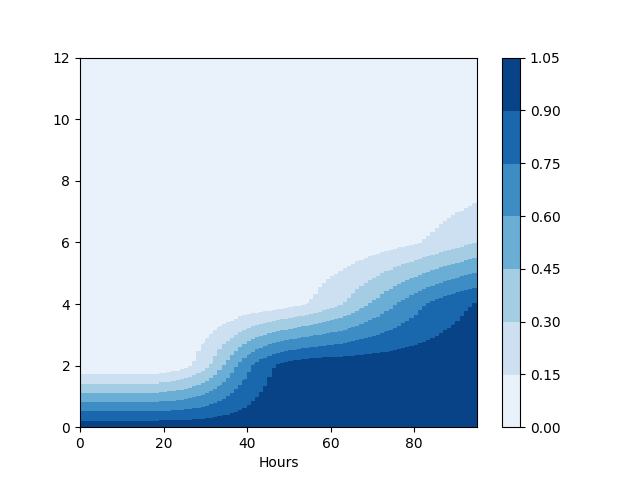
\includegraphics[scale=0.7]{brine_rise_snow_model}
\caption{Plot showing the development of the liquid fraction at different heights, simulating the harp.}
\label{modelski}
\end{figure}

This has some problems, biggest of which is the permeability value, which I will get back to. Another thing is that the rise is not as fast or high as the experiment showed, this is simply explained by the fact that this only takes into account the capillary pressure, and not the pressure created by gravity pushing the snow and ice down towards the water creating negative freeboard.\\
\\
What this model however is successfully showing is that the rise cannot be seen as a simple maximum rise, as it will not be uniformly distributed around the snow pack.\\
\\
For the permeability, the value is incredibly low, this is most likely due to me mixing up some orders. It could be that the assumed distribution is wrong, however, I tried raising the maximum and average size of the pores many times, and it did not change much. It could of course also be the correct value, as there is not much  research to build on here, this is very unlikely. Probably it is a function depending on temperature, grain size and density of the snow. To be certain about this, more experiments, in a controlled environment, is needed.\\
\\
Another thing is of course that this model was very machine heavy, but I am sure a similar model can be built with a lighter code.\\
\\
It is also worth noting that this assumes that the snowpack is filled with tubes that lead from the bottom and all the way up, an assumption that is not very realistic. Nonetheless, it does not change the result that much. If a more detailed model is needed it is possible to take this further, and instead of using the tube model of capillary pressure, use the radii of curvature and make an detailed analysis from this. It is not to complicated, but to much for a project of this size.

The wire harp could still be further improved, by for instance making it
possible to read out data, and check batteries without turning it off. If the
harps are to be used for snow-ice experiments I would recommend that they where
modified, to allow a higher impedance to be measured, as new snow will have a
much higher impedance than what we where dealing with, and much higher than
$17000 \Omega$. 

%\subsection{A Larger Perspective}
%Broad picture. Bind our findings with the motivation and importance of our data.



%------
%'Exeeds Standard' criteria for Report Grading:
%The Discussion provides meaningful and insightful analysis of the data, places the results in context, discusses implications and limitations of the findings, and draws conclusions supported by evidence
%------
